\begin{figure}[h]
    \centering
    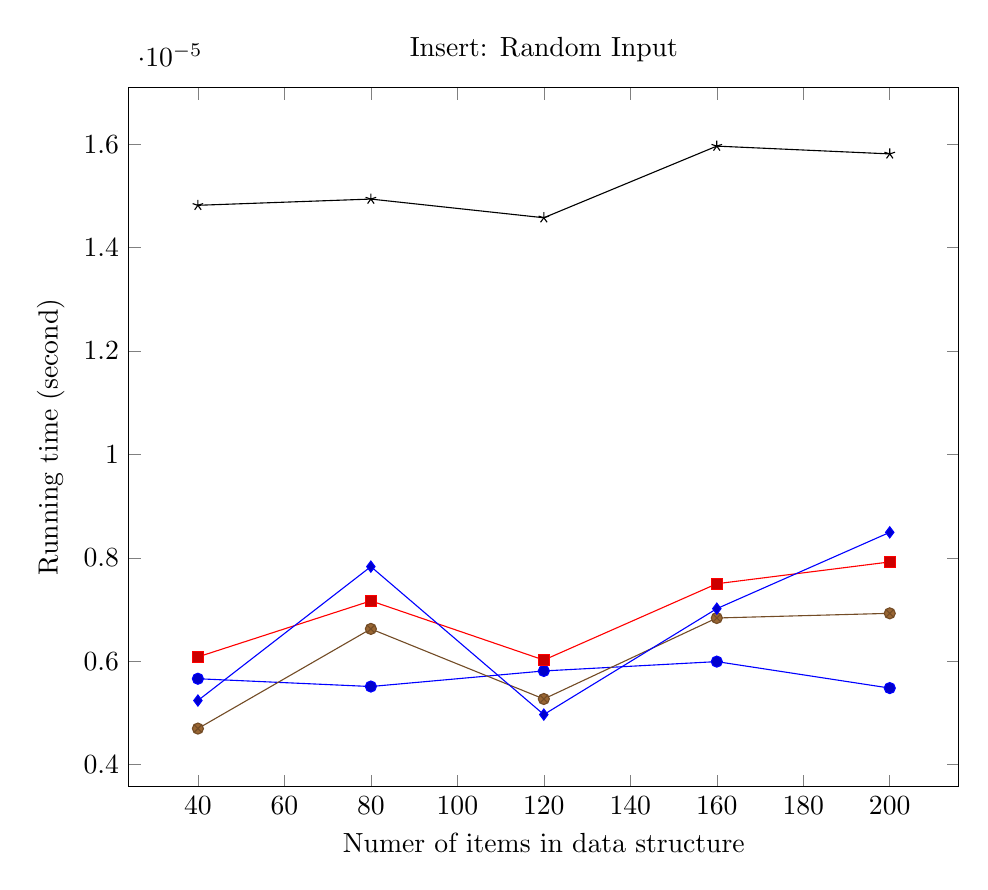
\begin{tikzpicture}
        \begin{axis}[
            xlabel={Numer of items in data structure},
            ylabel={Running time (second)},
            title={Insert: Random Input},
            width=\textwidth
        ]
		\addplot coordinates {
			(40, 5.662096330993905e-06)
			(80, 5.511508662436882e-06)
			(120, 5.812683999195656e-06)
			(160, 5.993389201464084e-06)
			(200, 5.4813911290807486e-06)
		};
		\addplot coordinates {
			(40, 6.083741802243025e-06)
			(80, 7.167973014787777e-06)
			(120, 6.023506735175488e-06)
			(160, 7.499265884902684e-06)
			(200, 7.920911356507076e-06)
		};
		\addplot coordinates {
			(40, 4.698335253294772e-06)
			(80, 6.6258574083377654e-06)
			(120, 5.270568393100916e-06)
			(160, 6.836680144317598e-06)
			(200, 6.927032745096539e-06)
		};
		\addplot coordinates {
			(40, 1.4817826568247482e-05)
			(80, 1.493829670273783e-05)
			(120, 1.4576886298911518e-05)
			(160, 1.5962292847859773e-05)
			(200, 1.581170517930275e-05)
		};
		\addplot coordinates {
			(40, 5.240450859389511e-06)
			(80, 7.830558755372864e-06)
			(120, 4.969393056342142e-06)
			(160, 7.017385346230754e-06)
			(200, 8.493144496313221e-06)
		};
        \legend{}
        \end{axis}
    \end{tikzpicture}
    \caption{Average of 0 operations, benchmarked every 0, starting at 0.}
\end{figure}